\documentclass[12pt]{article}
\usepackage{multirow}
\usepackage{graphicx}
\usepackage{wrapfig}
\usepackage[T2A]{fontenc}			% кодировка
\usepackage[utf8]{inputenc}			% кодировка исходного текста
\usepackage[english,russian]{babel}	% локализация и переносы
\usepackage{amsmath,amsfonts,amssymb,amsthm,mathtools} 
\usepackage{hyperref}
\usepackage[rgb]{xcolor}
\usepackage{wasysym}
\usepackage{fancyhdr}
\pagestyle{fancy}
\usepackage[left=3cm,right=3cm, top=3cm, bottom=3cm, bindingoffset=0cm]{geometry}
\usepackage{amsmath,amssymb,amsfonts,amsthm}
\usepackage{tikz}



\renewcommand{\maketitle}{%
	\noindent{\bfseries\scshape\large\@title\ \mdseries\upshape}\par
	\noindent {\large\itshape\@author}
	\vskip 2ex}
\makeatother
\def\dd#1#2{\frac{\partial#1}{\partial#2}}

\begin{document}
\begin{titlepage}
\begin{center}
\huge{Лабораторная работа № \textbf{4.2.3}}\\[1cm]\LARGE {Интерферометр Релея\\[7 cm]}
\end{center}

\begin{flushright}
\Large{Карманов Алексей\\752 группа}\\[9 cm]
\end{flushright}
\begin{center}
г.Долгопрудный\\
28.02.2019
\end{center}
\end{titlepage}
\fancyhead[L]
\indent \textbf{Цель работы:} Ознакомление с устройством и принципом действия интерферометра Релея и с его применением для измерения показателей преломления газов.\\[0.75 cm]
\indent \textbf{В работе используются:} Технический интерферометр ИТР-1, светофильтр, баллон с углекислым газом, сильфон, манометр, краны.\\
	\section{Описание установки}
\hspace{0.5 cm} Схема прибора представлена на рисунке 1 в вертикальной и горизонтальной проекциях. Лампа накаливания Л с помощью конденсора К ярко освещает узкую входную щель S, расположенную в фокусе объектива $O_1$. Коллиматор, состоящий из щели $S$ и объектива $O_1$, посылает параллельный пучок на диафрагму $D$ с двумя вертикальными щелями. Свет, дифрагируя на двойной щели проходит кювету $L$, состоящую из двух одинаковых стеклянных камер, в которые вводятся исследуемые газы. Кювета занимает только верхнюю часть пространства между объективами. За кюветой расположены две стеклянных пластинки $J$ и пластинка П. 
	
	Дифракционная картина, образующая в фокальной плоскости $F$ объектива $O_2$, рассматривается через окуляр $O$.
	
	\begin{figure}[h!]
		\begin{center}
			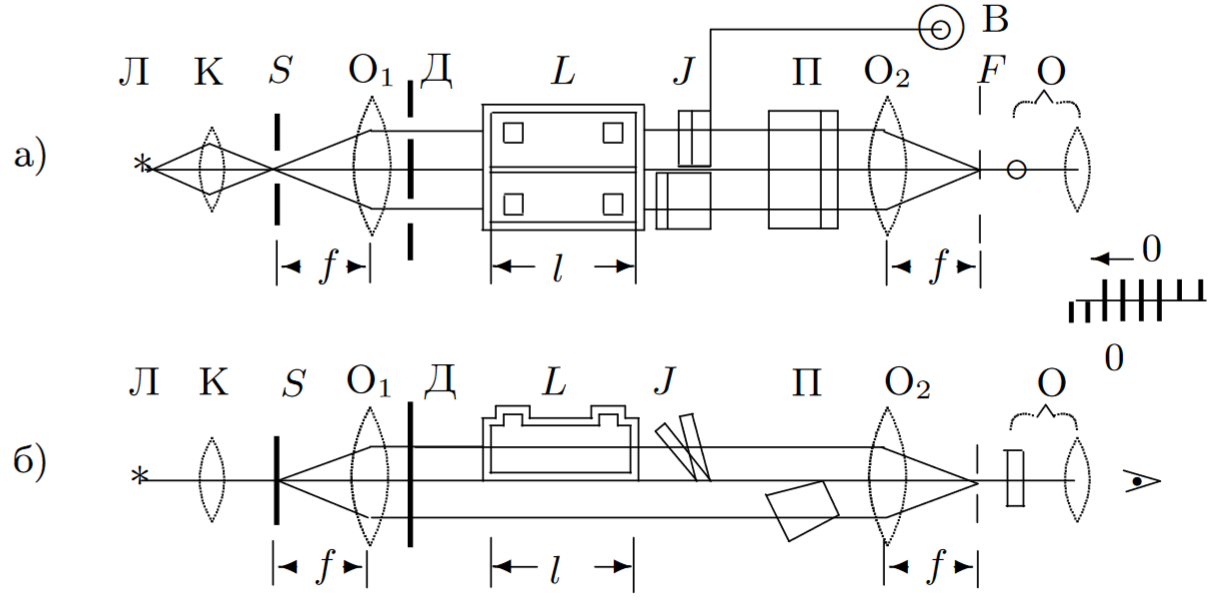
\includegraphics[width = \linewidth]{expsc}
			\caption{Схема установки: а) вид сверху, б) вид сбоку}
		\end{center}
	\end{figure}
	\newpage
	При заполнение камер газами с одинаковым показателем преломления $n$ системы полос совпадают. Разность хода $\Delta = \Delta n \cdot l$, возникает при прохождении света через камеры с разными газами и ведет к смещению полос. Смещение на одну полосу соответствует дополнительной разности хода $\Delta = \lambda$. Просчитав число полос между центрами можно рассчитать:
	\begin{equation}
	\delta n = \frac{\Delta}{l} = m\frac{\lambda}{l}
	\end{equation}
	
	\section{Зависимость показателя преломления газа от давления и температуры}
	Известно простое соотношение между показателем преломления газа и его плотностью:
	\begin{equation}
	n = \sqrt{\varepsilon} = \sqrt{1+4\pi N\alpha} \simeq 1 + 2\pi N \alpha
	\end{equation}
	Принимая во внимание $p = NkT$, получаем:
	\begin{equation}
	n - 1 = 2\pi\alpha\frac{P}{kT}
	\end{equation}
	Отсюда следует, что при постоянной температуре изменение показателя преломления $\delta n$ пропорционально изменению давления $\Delta P$.
	\begin{equation}
	\delta n = \frac{2\pi\alpha}{kT}\Delta P
	\end{equation}
	Длина кюветы $l = 10 \,\text{см}$, атмосферное давление $P = 101.2\cdot 10^3\,\text{Па}$, температура $T = 21 ^\circ C$. Прокалибруем установку в единицах $\lambda$. Для этого построим график смещения от номера полосы:\\
	
	
	\begin{table}[h!]
	\caption{Калибровка компенсатора}
\begin{tabular}{|l|l|l|l|l|l|l|l|l|l|l|l|}
\hline
m & 0    & 1   & 2    & 3   & 4    & 5   & 6    & 7    & 8   & 9    & 10   \\ \hline
d, mm & 3,05 & 3,40 & 3,75 & 4,10 & 4,43 & 4,70 & 5,05 & 5,38 & 5,70 & 6,05 & 6,35 \\ \hline
\end{tabular}
\end{table}
	\begin{figure}[h!]
		\begin{center}
			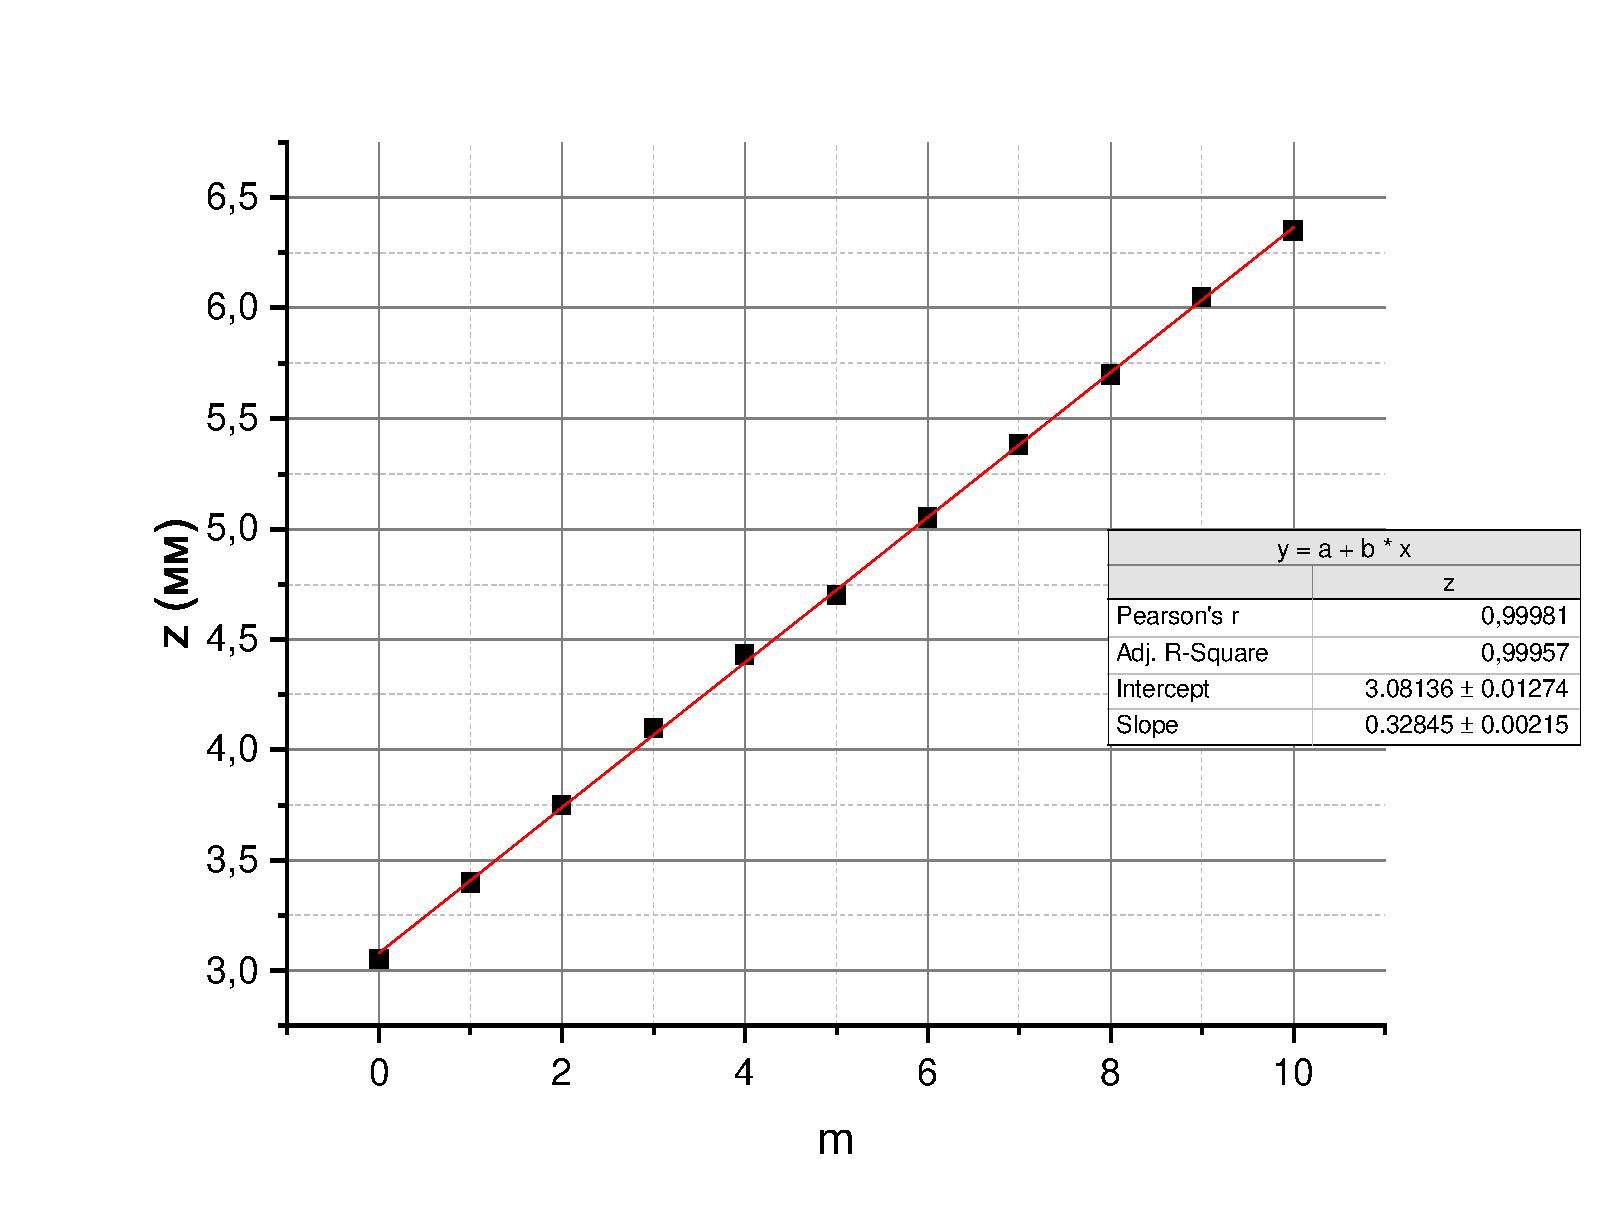
\includegraphics[width = 1.1\linewidth]{calibr}
			\caption{Зависимость смещения от номера полосы интерференционной картины}
		\end{center}
	\end{figure}
	\newpage
	Будем использовать калибровочный график для расчета $\delta n$. Таким образом построим график в координатах $\Delta n\left(\Delta P\right)$.\\
	
	\begin{table}[h!]
	\caption{Измерение раззницы показателей преломелния}
\begin{tabular}{|l|l|l|l|l|l|l|l|l|l|l|l|}
\hline
$\Delta P$ & -1000 & -800 & -600 & -400 & -200 & 0    & 200  & 400  & 600  & 800  & 1000 \\ \hline
z, мм  & 4,55  & 4,35 & 4,05 & 3,7  & 3,4  & 3,05 & 2,75 & 2,45 & 2,25 & 1,92 & 1,4  \\ \hline
\end{tabular}
\end{table}
	
	\begin{figure}[h!]
		\begin{center}
			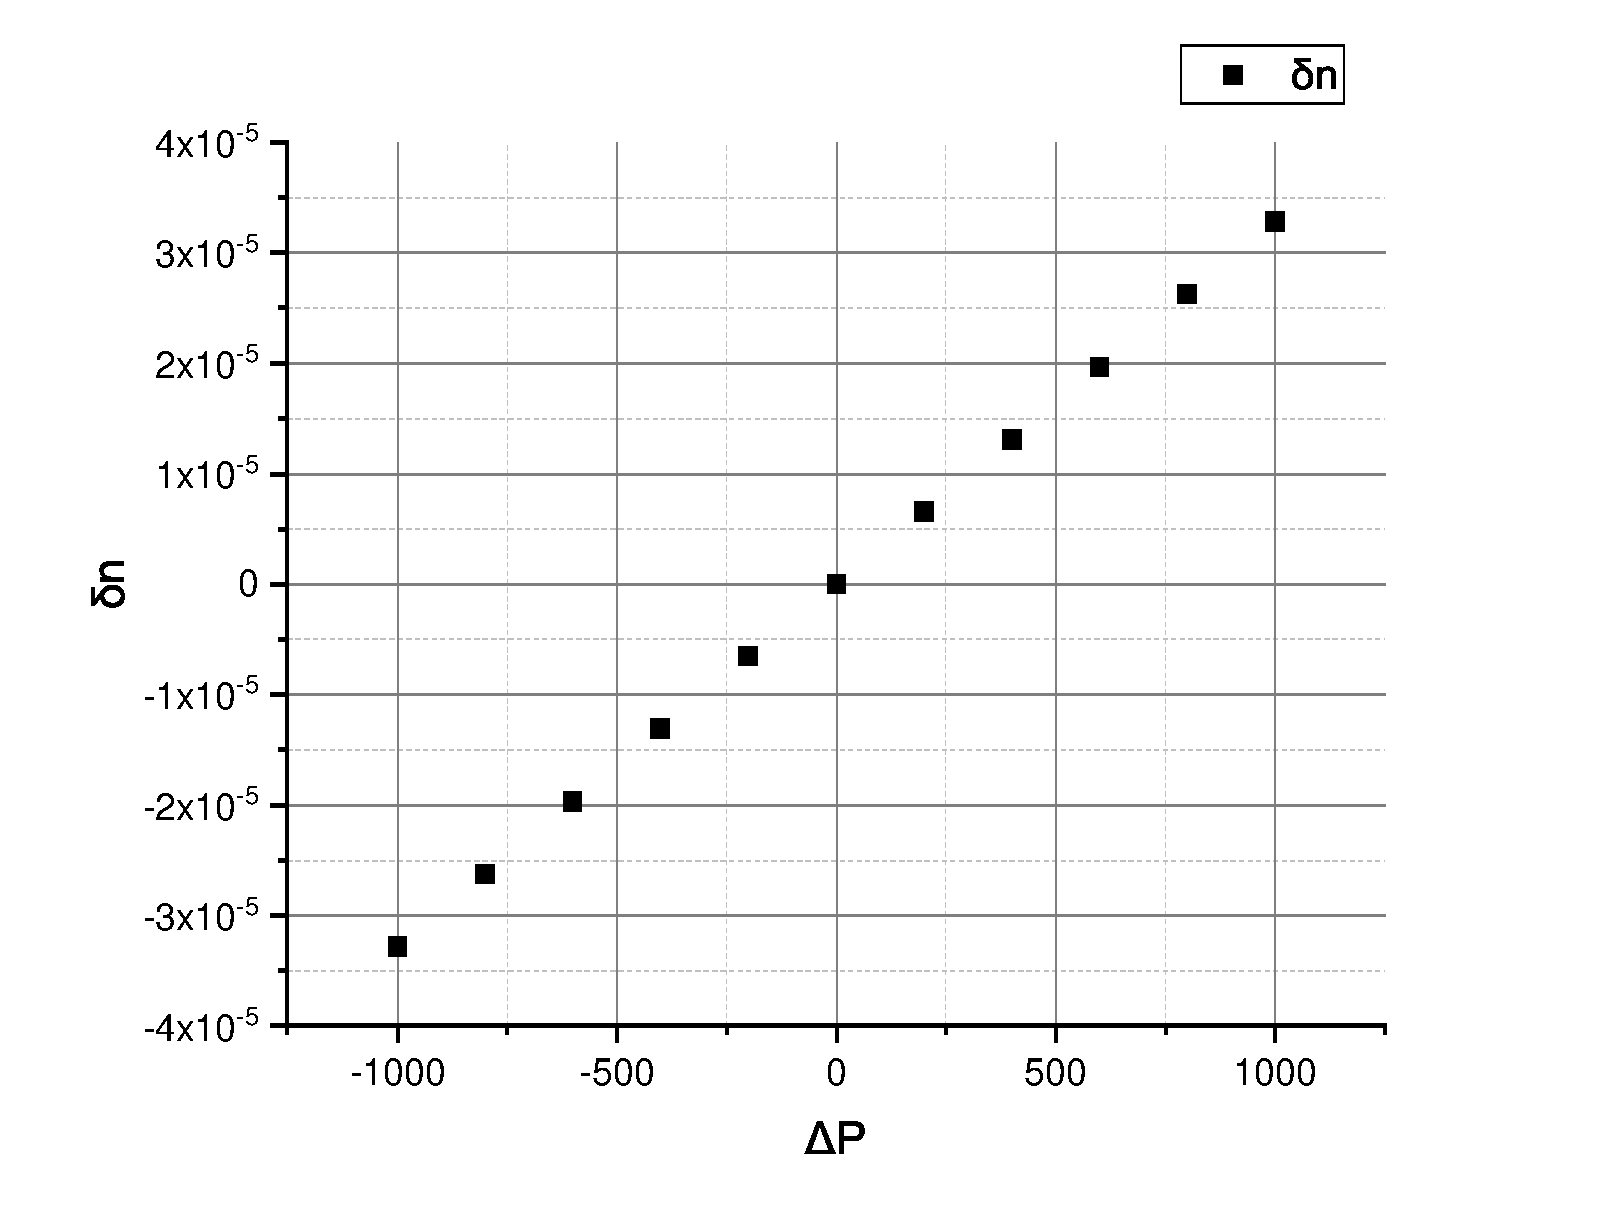
\includegraphics[width = \linewidth]{notp}
			\caption{Измерение разницы показателей преломления для воздуха под разным давлением}
		\end{center}
	\end{figure}
	
	Отсюда получаем показатель преломления воздуха. пересчитанный к нормальным условиям $ n_0 = 1.0003\pm 0.00005$, что сходится с табличным результатом в пределах погрешности($n_{0_{t}} = 1.0002929$)
	\newpage
\section{Расчет показателя преломления углекислоты}
	Теперь заполним кювету углекислым газом, и пронаблюдаем зависимость смещения компенсатора от времени:\\
	\begin{table}[h!]
	\caption{Установление равновесия}
\begin{tabular}{|l|l|l|l|l|l|l|l|l|l|l|l|}
\hline
t, мин & 0    & 1    & 2   & 3   & 4    & 5   & 6    & 7    & 8    & 9    & 10   \\ \hline
z, мм  & 10,1 & 8,95 & 8,1 & 7,5 & 6,95 & 6,5 & 6,15 & 5,55 & 5,25 & 5,02 & 4,85 \\ \hline
\end{tabular}
\end{table}
	
	\begin{figure}[h!]
		\begin{center}
			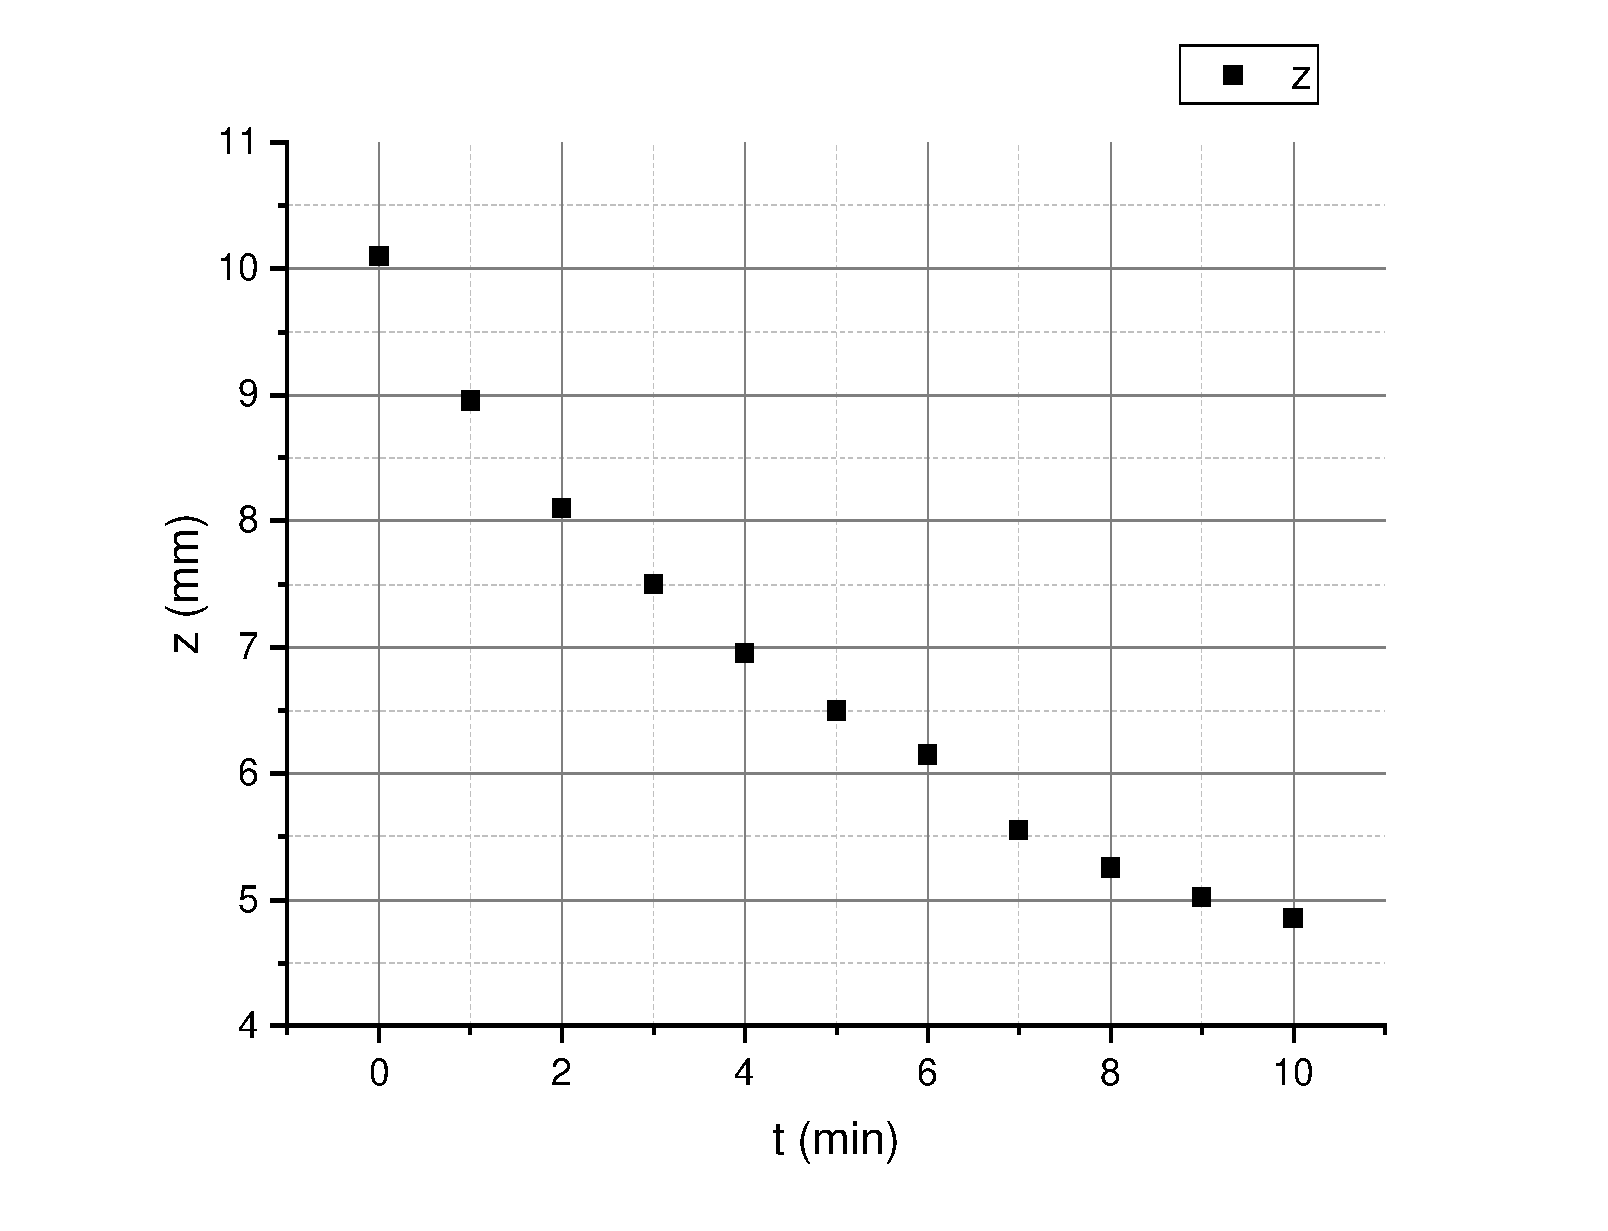
\includegraphics[width = \linewidth]{dt}
			\caption{Зависимость смещения компенсатора от времени}
		\end{center}
	\end{figure}
	\begin{table}[h!]
		\centering
		\caption{Расчет показателя преломления}
		\label{my-label}
		\begin{tabular}{|l|l|l|l|}
			\hline
			& d     & $\Delta n$ & n          \\ \hline
			1 & 10.55 & 0.000157   & 1.000457 \\ \hline
			2 & 10.46 & 0.000155   & 1.000455 \\ \hline
			3 & 10.48 & 0.000155   & 1.000455 \\ \hline
			4 & 10.46 & 0.000155   & 1.000455 \\ \hline
			5 & 10.53 & 0.000156   & 1.000456 \\ \hline
		\end{tabular}
	\end{table}
	
	\newpage
	
	
	Итого $n = 1.00045 \pm 0.00002$. Табличный показатель преломления для $CO_2$ $n_0 = 1.00045$, что также сходится с нашими измерениями.
	
	\section{Вывод}
	Интерферометр Релея позволяет измерять разность показателей преломления в двух кюветах с высокой точностью. Для таких измерений нужно поддерживать давление в кюветах и концентрацию газа постоянной, в противном случае точность и простота измерений значительно ухудшаются.
	

	


\end{document}